
\section{Implementierung in Python mit FEniCS}\label{Chapter_implementation}

In diesem Abschnitt möchten wir die Implementierung\footnote{Die Funktionsfähigkeit des Programms ist ausschließlich unter der Version Python 3.5, sowie den zugehörigen $FEniCS$-Paketen gewährleistet.} des Algorithmus \ref{2loopbfgs} in Python 3.5 mit Hilfe des Moduls FEniCS vorstellen. Im Folgenden werden wir die in den Dateien enthaltenen Kommentare nicht oder nicht in voller Länge in den Codeausschnitten aufführen, da wir Redundanz bei den Erklärungen vermeiden möchten. Selbstverständlich sind in den Quellcodes selber ausführliche Kommentierungen vorhanden, weshalb wir gerne auf diese verweisen. Die Implementierung in Python besteht zum Hauptteil aus den beiden Dateien
\begin{align*}
\textsf{shape\_main.py} \hspace{0.8cm} \textsf{shape\_bib.py}.
\end{align*}
Die Datei \textit{shape\_main.py} enthält hierbei den zusammenhängenden Hauptcode. Die Datei \textit{shape\_bib.py} ist eine Bibliothek, in welcher Funktionen zum Umgang mit Gittern, Berechnungen auf Formen, Löser für PDEs und der 2-Schleifen-L-BFGS-Algorithmus mit den damit verbundenen Objekten gebündelt sind. 
Beide Dateien, mit samt den von uns im nächsten Kapitel präsentierten Ergebnissen, sind in der Abgabe mit enthalten. Zusätzlich ist eine Testimplementierung der Objekte für das BFGS-Verfahren zur Lösung eines endlichdimensionalen Optimierungsproblems beigefügt, der zeigt, dass die Objekte alle das korrekte Verhalten haben. Die Berechnungen auf den Formen und das Lösen der PDEs wird mittels FEniCS geschehen.
FEniCS\footnote{Weitere Informationen sind unter https://fenicsproject.org/ zu finden.} ist eine frei zugängliches Programmpaket, welches ermöglicht, partielle Differentialgleichungen mit relativ geringem Aufwand zu lösen. Dabei bedient sich FEniCS der sogenannten \textit{Unified Form Language} (UFL), was die Grundlage zur Implementierung der PDE's in schwacher Formulierung darstellt, mehr hierzu bei \cite{Unifiedformlanguage}. 
Bevor wir uns der Lösung von PDE's und der Implementierung des L-BFGS-Algorithmus zuwenden, müssen wir zunächst klären, wie wir die notwendigen Gitter erzeugen und mit diesen umgehen.

\subsection{Gittererzeugung}
\label{meshgeneration}
Gitterdateien erzeugen wir mit Hilfe des offen zugänglichen Programms \textsf{Gmsh 3.0.6}\footnote{Weitere Informationen unter http://gmsh.info/.}. Hierbei muss  zunächst eine \textsf{.geo} Datei geschrieben werden. Wir zeigen dies am Beispiel eines kleinen Kreises, welcher für unsere.
Zunächst setzen wir die für unser Gitter relevanten Punkte in ein 3-dimensionales Koordinatensystem

\begin{lstlisting}
Point(1) = {0.0, 0.0, 0.0, 1.0};
Point(2) = {1.0, 0.0, 0.0, 1.0};
Point(3) = {0.0, 1.0, 0.0, 1.0};
Point(4) = {1.0, 1.0, 0.0, 1.0};
Point(5) = {0.5, 0.35, 0.0, 1.0};
Point(6) = {0.5, 0.5, 0.0, 1.0};
Point(7) = {0.5, 0.65, 0.0, 1.0};
\end{lstlisting}

Hierbei beschreiben die ersten 3 Einträge des Tupels die x-, y- und z-Koordinaten der Punkte, der vierte Eintrag gibt die sogenannte \textit{characteristic length} der Punkte an, was lediglich die Elementgröße des Punktes ist. Punkte 1 bis 4 werden dazu dienen das Einheitsquadrat im $\mathbb{R}^2$ zu definieren, Punkte 5 bis 7 werden einen Kreis mit Mittelpunkt $(0.5,0.5)$ definieren. Dies geschieht mittels der Befehle

\begin{lstlisting}
Line(1) = {1, 2};
Line(2) = {2, 4};
Line(3) = {4, 3};
Line(4) = {3, 1};

Circle(5) = {5, 6, 7};
Circle(6) = {7, 6, 5};
\end{lstlisting}

Da diese Befehle lediglich Linien und Halbkreise aus den eingegebenen Punkten definieren, ist es nötig mittels eines \textsf{Loop}-Befehls diese zu einer gemeinsamen Form zu verbinden.

\begin{lstlisting}
Line Loop(1) = {1, 2, 3, 4};
Line Loop(2) = {5, 6};
\end{lstlisting}

Um innere und äußere Gebiete, welche durch Abgrenzung mittels des Kreises definiert sind, zu markieren, setzen wir diese als \textsf{Plane Line} fest. Die erste Zahl gibt jeweils die Nummer des \textsf{Line Loops} des äußeren Randes, die zweite die des inneren Randes an.

\begin{lstlisting}
Plane Surface(1) = {1, 2};
Plane Surface(2) = {2};
\end{lstlisting}

Weil wir später in der Implementierung auf die Ränder bzw. Formen zugreifen möchten, ist es abschließend noch nötig diese als sogenannte \textsf{Physical Lines} und \textsf{Physical Surfaces} zu definieren. 

\begin{lstlisting}
Physical Line(1) = {1};
Physical Line(2) = {2};
Physical Line(3) = {3};
Physical Line(4) = {4};
Physical Line(5) = {5};
Physical Line(6) = {6};

Physical Surface(1) = {1};
Physical Surface(2) = {2};
\end{lstlisting}

Die so geschriebene \textsf{.geo}-Datei wird nun mit Hilfe des Programms \textsf{Gmsh} in der Konsole mit dem Kommando

\begin{center}
\textsf{gmsh mesh\_smallercircle.geo -2 -clscale 0.1}
\end{center}

in eine \textsf{.msh} Datei konvertiert. Dabei ist \textsf{mesh\_smallercircle.geo}
der Name der gespeicherten \textsf{.geo}-Datei, \textsf{-2} die Dimension des erzeugten Gitters und \textsf{0.1} die Feinheit des Gitters. Um diese Datei für FEniCS nutzbar zu machen, konvertieren wir diese mit Hilfe des Dolfin-Befehls

\begin{center}
\textsf{dolfin-convert mesh\_smallercircle.msh mesh\_smallercircle.xml}
\end{center}

wobei der erste Eingabewert der Name der \textsf{.msh}-Datei ist, und der zweite der Name der erzeugten \textsf{.xml}-Datei. Hierbei werden außerdem neben dem bloßen Mesh auch eine \textsf{facet\_region.xml}-Datei erstellt, mit welcher man die Ränder initialisieren kann, sowie eine \textsf{physical\_region.xml}-Datei, welche zur Initialisierung der Gebiete des Inneren und Äußeren der Form dient.
Beispielgitter finden sich im nächsten Kapitel über die Resultate, etwa in \ref{Meshes}.

\subsection{Die Bibliothek shape\_bib}
\subsubsection{Die MeshData-Klasse}
\label{meshdataclass}
Nun besitzen wir die nötigen Gitterdateien, um auf diesen Formoptimierung zu betreiben. Wir stellen kurz vor, mit welchen Objekten und Funktionen wir auf diesen operieren. Eines der beiden zentralen Klassen des Optimierungsprogramms ist die sogenannte \textit{MeshData-Klasse}. 

\begin{lstlisting}
class MeshData:

    # Objekt mit allen Daten des Gitters
    def __init__(self, mesh, subdomains, boundaries, ind):

        # FEniCS Mesh
        self.mesh = mesh

        # FEniCS Subdomains
        self.subdomains = subdomains

        # FEniCS Boundaries
        self.boundaries = boundaries

        # Indizes der Knotenpunkte mit Traeger nicht 
        # am inneren Rand
        self.indNotIntBoundary = ind
\end{lstlisting}

In einem Objekt dieser Klasse werden sowohl das Gitter, als auch die Gebiete und Ränder bzw. Formen gespeichert. Weiterhin benötigen wir für spätere folgende Berechnungen auch die Indizes der Knotenpunkte (engl. \textit{Vertices}), welche keinen Träger am inneren Rand haben, gespeichert. Die Initialisierung erfolgt mit der von uns implementierten Funktion 
\begin{center}
\textsf{load\_mesh(Name)},
\end{center} wobei \textsf{Name} der Name der Mesh-Datei ohne \textsf{.xml}-Endung ist. Die \textsf{subdomains} und \textsf{boundaries} werden jeweils als ein sogenannte \textsf{MeshFunction} initialisiert. Dies sind Objekte einer in FEniCS implementierten Klasse, welche als Array im \textsf{i}-ten Eintrag die Nummer der \textsf{subdomain} bzw. der \textsf{boundary} zurückgeben, welche den Nummern der \textsf{Physical Surface} bzw. \textsf
{Physical Line}  in der \textsf{.geo}-Datei entsprechen. Diese Initialisierungen geschehen über die Befehle

\begin{lstlisting}
mesh 	     = Mesh(path_meshFile + ".xml")
subdomains = MeshFunction("size_t", mesh,
                          path_meshFile + "_physical_region.xml")
boundaries = MeshFunction("size_t", mesh, 
                          path_meshFile + "_facet_region.xml")
ind        = __get_index_not_interior_boundary(mesh, subdomains, 
                                               boundaries)  
\end{lstlisting}
wobei \textsf{Mesh} als Eingabe den Pfad zur \textsf{.xml}-Datei enthält. Die Meshfunktionen erhalten neben dem \textsf{mesh}-Objekt den Typ der Funktion, in diesem Fall \textsf{size\_t}, und die Pfade zu den jeweiligen Dateien \textsf{\_physical\_region.xml} und \textsf{\_facet\_region.xml}. Es bleibt noch, die Indexliste der Indizes mit Träger nicht am Inneren Rand zu initialisieren. Um diese Indexliste zu erzeugen haben wir die Funktion 
\begin{align*}
\textsf{\_\_get\_index\_not\_interior\_boundary(mesh, subdomains, 
boundaries, interior = True)}  
\end{align*}
implementiert. Als Input erhält sie die oben gezeigten Objekte, falls \textsf{interior = True} eingestellt ist, so gibt die Funktion die Liste mit Indizes ohne Träger am inneren Rand wieder. Wir möchten an dieser Stelle anmerken, dass Indizes auch mehrfach vorkommen, was für unser Programm kein Problem darstellt und bei Bedarf verbessert werden kann. Ist der Parameter \textsf{interior = False}, so gibt die Funktion eine Liste mit den Indizes der Knotenpunkte genau des inneren Randes wieder. Dies spart uns die Implementierung einer weiteren Funktion. Das erzeugen der Liste basiert auf Iterationen durch Facetten des Randes, deren Knoten und den benachbarten Knoten. Diese aufwändige Iteration ist nötig, da die Indizierung der Facetten in der Meshfunktion des Randes in FEniCS nicht mit den Indizes der Mesh's übereinstimmen. Für die genaue Implementierung verweisen wir auf den von uns beigefügten Code. 

\subsubsection{Berechnungen in der shape\_bib}\label{Berechnung_bib}
 Der Hauptanteil der Berechnungen besteht in dem Lösen von partiellen Differentialgleichungen. Die Gleichungen, welche wir für die Formoptimierung lösen müssen, haben wir in den vorigen Kapiteln eingeführt. Dabei handelt es sich um die Poisson-Zustandsgleichung mit Interface Condition aus unserem Modellproblem \ref{Modellproblem}, die zugehörige adjungierte Gleichung \ref{Modelladjoint}, und die lineare Elastizitätsgleichung \ref{linelas}, welche uns einen Formgradienten liefern wird. Wir möchten exemplarisch an der implementierten Funktion zur Lösung der linearen Elastizitätsgleichung zeigen, wie dies in FEniCS praktisch passiert. Für die beiden anderen Gleichungen wird analog vorgegangen, hierbei verweisen wir auf unseren Quellcode. Die Lösung der Gleichungen wird über die Funktionen 
\begin{lstlisting}
solve_state(meshData, fValues)
solve_adjoint(meshData, y, z)
solve_linelas(meshData, p, y, z, fValues, 
	            mu_elas, nu, zeroed = True)
\end{lstlisting}
zurückgegeben, wobei jede Funktion ein Objekt der \textsf{MeshData}-Klasse erhält, sowie die nötigen Funktionen aus den oben genannten Gleichungen, welche als sogenannte \textit{FEniCS-Funktionen} initialisiert sind. Der Löser der linearen Elastizitätsgleichung benötigt weiterhin die in \ref{loclame} eingeführten lokal-variierenden Lamé-Parameter, sowie den Parameter der Perimeter-Regularisierung \textsf{nu}. Zusätzlich gibt dieser die Norm des Objekts, welches die Formableitung als Operator auf dem Raum der Testfunktionen repräsentiert, als zweiten Return wieder, mehr hierzu im weiteren Verlauf bei \ref{felas}. Die Einstellung \textsf{zeroed = True} bewirkt, dass bei Lösen der Gleichung die Werte der Punkte ohne Träger am inneren Rand auf 0 gesetzt werden, was eine Instabilität des Verfahrens vermeidet. Wir vermuten, dass es sich bei den Instabilitäten um Rundungs- und/ oder Diskretisierungsfehler handelt, siehe \cite{bfgs2}, Abschnitt 5. Die genaue Ursache der Fehler ist jedoch nicht sicher geklärt. 

Wie oben schon erwähnt, sind die Funktionen \textsf{p, y, z} FEniCS-Funktionen. 
Skalarwertige FEniCS-Funktionen \textsf{f} auf dem Gitter \textsf{meshData.mesh} werden beispielsweise mit
\begin{lstlisting}
V = FunctionSpace(meshData.mesh, "P", 1)
f = Function(V)
\end{lstlisting}
initialisiert. Um die lineare Elastizitätsgleichung zu lösen, müssen wir zunächst den zugehörigen Funktionenraum angeben, was durch
\begin{lstlisting}
V = VectorFunctionSpace(meshData.mesh, "P", 1, dim=2)
\end{lstlisting}
geschieht. Da die Lösung eine vektorwertige Funktion ist, ist es für FEniCS notwendig die Dimension explizit anzugeben. Die Parameter \textsf{"P"} und \textsf{1} geben an, dass die Werte zwischen den Gitterpunkten mittels einer Polynominterpolation vom Grad 1 erzeugt werden. Hier sind weitere Möglichkeiten zur Interpolation gegeben, siehe \cite{fenics}. Um die Gleichung aufzustellen, müssen wir Randwerte festlegen. Für die Dirichlet-Nullrandwerte geschieht dies über den Befehl
\begin{lstlisting}
u_out = Constant((0.0, 0.0))
bcs = [DirichletBC(V, u_out, 
                   meshData.boundaries, i) for i in range (1, 5) ]
\end{lstlisting}
wobei \textsf{i} über die Nummern der äußeren Ränder läuft. FEniCS unterscheidet beim Lösen von Differentialgleichungen zwischen Testfunktionen und der Lösungsfunktion. Der Unterschied zu normalen Funktionen ist, dass mit diesen bei dem Assemblieren der schwachen Formulierung die Terme, etwa die Bilinearform $a$ weiter unten, nicht ausgewertet werden können, im Unterschied zu regulären FEniCS-Funktionen. Wir initialisieren diese mittels
\begin{lstlisting}
U = TrialFunction(V)
v = TestFunction(V)
\end{lstlisting}
wobei \textsf{U} die Lösung, also das Gradientenvektorfeld in Domaindarstellung, und \textsf{v} stellvertretend für die zum Raum \textsf{V} gehörenden Testfunktionen steht. Nun wird die linke und rechte Seite der Gleichung aufgestellt:
\begin{lstlisting}
LHS    = bilin_a(meshData, U, v, mu_elas)
F_elas = shape_deriv(meshData, p, y, z, fValues, nu, v)
\end{lstlisting}
Hierbei ist \textsf{bilin\_a} die aus \ref{finalformgradient} bekannte Bilinearform, und \textsf{shape\_deriv} die Formableitung $D\mathcal{J}(\Omega)[V]$ als Summe von den Darstellungen \ref{shapederivsurfacetarget} und \ref{shapederivsurfaceperimeter}. Beides wird in der für FEniCS typischen Weise assembliert, wobei wir dies exemplarisch an der Bilinearform \textsf{bilin\_a} aufzeigen: \label{bilina}
\begin{lstlisting}
def bilin_a(meshData, U, V, mu_elas):

    dx = Measure("dx", domain=meshData.mesh, 
                 subdomain_data=meshData.subdomains)

    epsilon_V = sym(nabla_grad(V))
    sigma_U   = 2.0*mu_elas*sym(nabla_grad(U))

    a     = inner(sigma_U, epsilon_V)*dx('everywhere')
    value = assemble(a)

    return value

\end{lstlisting}
Input sind ein Objekt der \textsf{MeshData}-Klasse, sowie zwei FEniCS Funktionen \textsf{U, V} und die lokal-variierenden Lamé-Parameter \textsf{mu\_elas}. Hier kommt die Stärke von FEniCS zur Geltung, nämlich die Verwendung der eingangs erwähnten \textit{Unified Form Language}. Die hier initialisierten Objekte sind exakt die Objekte, welche in der schwachen Formulierung der Gleichung \ref{linelas}  auftauchen, was der mathematischen Schreibweise sehr nahe steht, und somit die Lesbarkeit und Übersicht deutlich erhöht. Es ist lediglich notwendig die Objekte abschließend zu assemblieren um einen Wert zu erhalten. Dies geschieht mit dem Befehl \textsf{assemble}. Genau auf selbige Weise wird die Formableitung \textsf{shape\_deriv} aufgebaut, weshalb wir hier auf den Quellcode verweisen. Da die Angabe der programmiertechnischen Details der Objekte der UFL den Rahmen dieser Arbeit sprengen würde, verweisen wir für den interessierten Leser auf \cite{fenics} und \cite{Unifiedformlanguage}.

Es bedarf nur noch dem Initialisieren der Randbedingungen für die assemblierten Objekte, bevor wir die lineare Elastizitätsgleichung lösen. Zuvor bauen wir noch die Option ein, die Werte, welche nicht am Träger des inneren Randes sind, auf Null zu setzen.

\begin{lstlisting}
if(zeroed): F_elas[meshData.indNotIntBoundary] = 0.0

for bc in bcs:
    bc.apply(LHS)
    bc.apply(F_elas)
\end{lstlisting}

Das lösen der nun aufgebauten Gleichung erfolgt mit dem Befehl.
\begin{lstlisting}
U = Function(V, name="deformation_vec")
solve(LHS, U.vector(), F_elas)

# Rueckgabe des Deformationsvektorfeldes U und der Abbruchbedingung
return U, nrm_f_elas

\end{lstlisting}

Zu beachten ist, dass wir \textsf{U} als \textsf{.vector()} Objekt übergeben. Diese Objekte lassen Arithmetik, wie beispielsweise das Initialisieren einzelner Werte an Knoten des Gitters für die FEniCS-Funktion, zu. Dies werden wir bei der Implementierung des BFGS-Schrittes maßgeblich verwenden. Das Objekt \textsf{F\_elas} ist bereits von diesem Typ, da wir nicht mit einer bestimmten Richtung, sondern mit einer \textsf{TestFunction} initialisiert haben, weshalb wir hier keinen Befehl benötigen. Das so entstandene Objekt ist also keine skalare Größe, sondern lässt sich als
\begin{align}\label{felas}
	D\mathcal{J}(\Omega)[\varphi_i] \; \hat{=}\; \textsf{F\_elas.get\_local()[i]}
\end{align}
interpretieren, wobei $\varphi_i$ polynomielle Basisfunktionen vom Grad 1 auf dem Gitter sind, welches $\Omega$ repräsentiert. Auf diese Weise lässt sich $D\mathcal{J}(\Omega)[\cdot]$ über \textsf{F\_elas} als skalarwertige Funktion auf dem initialisierten Gitter auffassen, wobei die jeweiligen Werte des Knoten mit Index \textsf{i} genau den Ableitungen $D\mathcal{J}(\Omega)[\varphi_i]$ entsprechen. Dies ermöglicht es uns, die $\mathcal{L}^2$-Norm des so zur Formableitung assoziierten Objekts zu bilden, welche genau der zweite Return \textsf{nrm\_f\_elas} ist. 
Die Größe dieser Norm wird bei uns als Ausstiegskriterium sowohl bei dem Gradienten-, als auch bei dem L-BFGS-Verfahren Verwendung finden.
Wir warnen den Leser an dieser Stelle, dass die obige Indizierung der Gitterpunkte $i$ und somit der Basisfunktionen $\varphi_i$ im Allgemeinen nicht mit der Indizierung der Werte der FEniCS-Funktionen auf dem Gitter, welche \textit{Degrees of freedom (DOF)} genannt werden, und somit nicht mit \textsf{F\_elas.get\_local()[i]} übereinstimmen. Dennoch lässt sich eine entsprechende Bijektion finden, welche in \textsf{Dolfin} mit dem Befehl \textsf{Dolfin.vertex\_to\_dof\_map(V)} erzeugt wird. Diese wird bei uns zum berechnen eines nötigen Formabstandes verwendet, auf welchen wir nun zu sprechen kommen.

Die Distanz zweier Formen werden wir mit der Funktion
\begin{align}\label{distfktdef}
	d_{shp}(\partial\Omega_1, \partial\Omega_2) := \underset{\partial\Omega_2}{\int} \underset{y\in\partial\Omega_1}{\min} \vert\vert x - y \vert\vert dx
\end{align}
messen. Diese Distanzfunktion wird bei uns lediglich als Ersatz für den Abstand zweier Formen im Formraum verwendet, welchen man mittels Geodätischer definieren kann, und ist eine Abwandlung des Hadamard-Abstandes. Um Geodätische zu bestimmen wäre es nötig eine weitere Differentialgleichung zu lösen, was wir vom Aufwand für nicht vertretbar halten, obwohl dies die korrektere Variante zur Abstandsmessung wäre. Wir bemerken außerdem, dass die oben definierte Abstandfunktion $d_{shp}$ nicht symmetrisch ist, was sich auch anhand der von uns implementierten Beispielformen leicht vorführen lässt. Die Auswertung dieser Distanzfunktion passiert über die von uns implementierte Funktion
\begin{lstlisting}
mesh_distance(mesh1, mesh2)
\end{lstlisting}
wobei \textsf{mesh1, mesh2} Objekte der \textsf{MeshData}-Klasse sein müssen. Die eigentliche Berechnung der Minima geschieht über Iteration aller sich auf den jeweiligen Boundaries befindlichen Punkte, deren Vertex-Indizes wir aus den Facettenindizes beispielsweise mittels     
\begin{center}
\textsf{\_\_get\_index\_not\_interior\_boundary(mesh2.mesh, mesh2.subdomains, mesh2.boundaries, interior = False)}
\end{center}
erhalten. Wie bei der linearen Elastizitätsgleichung erwähnt, lässt sich die Liste der Minima der einzelnen Punkte $x$ nicht ohne weiteres als FEniCS-Funktion initialisieren, da der angesprochene Unterschied der Indizierung der Gitterpunkte und DOFs Probleme bereitet. An dieser Stelle kommt die \textsf{vertex\_to\_dof\_map} zum tragen. Abschließend findet eine zu \ref{bilina} ähnliche Assemblierung des Integrals statt, welche uns den Abstandwert als Return liefert. 

\subsubsection{Die BFGS-Memory-Klasse}

Die von uns bisher eingeführten Objekte würde schon ausreichen, um ein Verfahren auf Basis des Gradientenabstiegs zu programmieren. Wir möchten jedoch als Ziel dieser Arbeit einen Schritt weiter gehen, und den L-BFGS-Algorithmus implementieren. Das Hauptproblem bei dem Verfahren besteht darin, sich eine Möglichkeit schaffen, mit dessen Hilfe man die Gradienten- und Deformationsfelder bequem speichern und updaten kann, da wir ja nur eine \textit{limited memory} besitzen. Hierzu entwerfen wir die zweite wichtige Klasse in unserem Programm, die sogenannte \textsf{bfgs\_memory}-Klasse. Diese ist wie folgt aufgebaut, wobei wir im Programm selber noch Initialisierungsfehler mit Warnungen an künftige weitere Verwender eingebaut haben, siehe den Quellcode:

\begin{lstlisting}
class bfgs_memory:

    def __init__(self, gradient, deformation, length, step_nr):

        # Liste von Gradientenvektorfeldern
        self.gradient = gradient

        # Liste von Deformationsvektorfeldern
        self.deformation = deformation

        # Anzahl der gespeicherten letzten Schritte
        self.length = length

        # Anzahl der bereits ausgefuehrten l-BFGS-Schritte
        self.step_nr = step_nr
\end{lstlisting}

Diese Klasse besteht aus zwei Listen von Arrays, \textsf{gradient} und \textsf{deformation}, und zwei Integer-Werten \textsf{length} und \textsf{step\_nr}. 
\textsf{length} ist der Parameter, welche die Anzahl der gespeicherten vorherigen Schritte im L-BFGS-Verfahren angibt, und somit die Länge der Liste der Arrays bestimmt. \textsf{step\_nr} ist ein Counter, welcher die Schritte des L-BFGS-Verfahrens zählt. 

Die Gradienten und Deformationen werden als Arrays, welche jeweils die DOF-Werte der FEniCS-Funktionen der Gradienten- und Deformationsvektorfelder enthalten, dem Alter her aufsteigend gespeichert. Das bedeutet beispielsweise, dass mit 
\begin{center}
	\textsf{bfgs\_memory.gradient[1]}
\end{center} 
die Liste der DOF-Werte des vorletzten Gradientenvektorfeldes abgerufen werden. Die Speicherung als Array, und nicht als FEniCS-Funktion, ist nötig, da wir damit den Transport der Vektorfelder umgehen. FEniCS-Funktionen sind unweigerlich an das Gitter, auf dem sie initialisiert wurden, gebunden, und eine Änderung des zugrunde liegenden Gitters macht die Funktionen unbrauchbar. Da wir die Indizierung der Knoten, und damit die der DOFs, nicht durch Deformationen verändern, entkoppeln wir die Funktionswerte von dem Gitter, indem wir ausschließlich diese nach der DOF Indizierung speichern. Damit erreichen wir den vereinfachten Transport nach \cite{diffusion}, Abschnitt 4. 
Anschließend  lässt sich bei Bedarf mit diesen Daten eine neue FEniCS-Funktion auf einem neuen Gitter initialisieren.
\begin{lstlisting}
def initialize_grad(self, meshData, i):

    if isinstance(meshData, MeshData): pass
    else: raise SystemExit("initialize_grad benoetigt Objekt der MeshData-			 						   Klasse als Input!")

    V = VectorFunctionSpace(meshData.mesh, "P", 1, dim=2)
    f = Function(V)
    f.vector()[:] = self.gradient[i]
    return f
\end{lstlisting}
wobei es wichtig ist, ein Objekt der \textsf{MeshData}-Klasse zu übergeben. Es ist wichtig zu beachten, dass die Initialisierung von Werten in die FEniCS-Funktion ausschließlich durch einen kompletten Slice-Befehl auf allen Gitterpunkten erfolgen sollte, da FEniCS sonst eine automatische Konvertierung der Funktion durchführt und diese für einige spätere Berechnungen unbrauchbar macht. Da wie angesprochen die Indizierung invariant bei Verschiebung ist, ist dies kein Problem.

Um die Memory zu updaten, haben wir eine Update-Funktion implementiert, welche 
den ältesten Wert, sobald die Anzahl \textsf{length} an gespeicherten Einträgen überschritten wird, löscht, und alle anderen dem Index nach um 1 aufrückt. 

\begin{lstlisting}
def update_grad(self, upd_grad):
    
    for i in range(self.length-1): 
      	self.gradient[-(i+1)]  = self.gradient[-(i+2)]
    
    self.gradient[0] = upd_grad
\end{lstlisting}

Wir wollen anmerken, dass sich diese Klasse natürlich auch direkt für die Implementierung von anderen Limited-Memory-Verfahren weiterverwenden ließe. 
Mit Hilfe dieser Klasse lässt sich nun ein L-BFGS-Schritt nach dem 2-Schleifen-Algorithmus \ref{2loopbfgs} implementieren. Dies haben wir mit der Funktion 
\begin{center}
\textsf{bfgs\_step(meshData, memory, mu\_elas, q\_target)}
\end{center} 
getan. Diese Funktion benötigt als Input zum einen ein Objekt der  \textsf{MeshData}-Klasse, auf der die FEniCS-Funktionen initialisiert, und die Bilinearform \textsf{bilin\_a} ausgewertet werden. Für die Bilinearform werden zudem die Lamé-Parameter \textsf{mu\_elas} benötigt. Weiterhin wird eine \textsf{bfgs\_memory} verlangt, mit deren Daten die genannten Funktionen erzeugt werden. Die von uns in vorigen Beispielen erläuterte Arithmetik mit FEniCS-Funktionen kommt hierbei zum tragen. Da dies zu langen Codesequenzen führt, verweisen wir für die genaue Implementierung auf den beiliegenden Quellcode. \textsf{q\_target} ist hier ein Array mit den DOF-Werten einer FEniCS-Funktion, in welcher der in dem Schritt berechnete approximierte Hesse-Operator ausgewertet wird. So gibt die Funktion \textsf{bfgs\_step} eine vektorwertige FEniCS-Funktion zurück, welche als Deformationsvektorfeld dienen kann, und mit
\begin{center}
$-B_k^{-1} q_{target} \; \hat{=} \; \textsf{bfgs\_step(meshData, memory, mu\_elas, q\_target)}$
\end{center}
identifiziert werden kann, falls $k>0$. Im Falle, dass die Memory noch leer ist, und kein Schritt zuvor durchgeführt wurde, gibt die Funktion das negative Eingabevektorfeld \textsf{$-q_{target}$} wieder. Wir möchten den Leser darauf aufmerksam machen, dass die Position der in der Memory gespeicherten Gradienten und Deformationen für die korrekte Berechnung des Schrittes essentiell sind. Befindet man sich in Schritt $k$, so muss der Eintrag \textsf{memory.gradient[0]} der $k$'te Gradient sein, und \textsf{memory.deformation[0]} die zuvor im Schritt $k-1$ berechnete Deformation $S_{k-1}$. D.h. die Memory muss auf dem aktuellst möglichen Stand sein. Jetzt besitzen wir das gesamte Rüstzeug, um in der Hauptdatei die Bausteine miteinander zu vernetzen.

\subsection{Das Hauptprogramm shape\_main}
\subsubsection{Der Hauptalgorithmus und Einstellungen}

Die von uns eingeführten Funktionen und Objekte lassen sich nun auf bequeme Weise miteinander in Verbindung bringen. Die Hauptdatei führt, je nach Einstellung der Parameter, eine Formoptimierung mit in der Datei verstellbarem Verfahren und Gittern durch. Zunächst zur Auswahl der Gitter; diese müssen in der Konsole bei Aufruf des Programms als \textsf{integer}-Parameter mit dem Befehl
\begin{center}
 \textsf{python3.5 shape\_main.py -m 9}
\end{center}
übergeben werden, wobei wir hier das Beispielgitterpaar 9, welches für die Gitterkombination
\begin{center}
\textsf{("mesh\_fine\_smallercircle", "mesh\_fine\_broken\_donut")}
\end{center}
steht, verwendet wird. Eine Liste der Gitter kann mit dem Befehl 
\begin{center}
 \textsf{python3.5 shape\_main.py -h}
\end{center}
angezeigt werden. Das Startgitter wäre in diesem Fall das eines fein aufgelösten kleinen Kreises, der zweite Eintrag das Zielgitter eines fein aufgelösten, nierenartigen Form, zu sehen in Abbildung \ref{Meshes}.

Wir haben bei der Wahl des Gitters außerdem die Option eingebaut, bei der man als Startgitter mit einer in jedem Punkt am Rand unabhängig normalverteilt gestörten Version des ersten Eintrags der Gitterpaare startet, und als Zielgitter das ungestörte Startgitter verwendet. Diese Option lässt sich mit den Parametern \textsf{Pertubation} und \textsf{sigma} steuern, wobei der erste Parameter diesen Optimierungsfall bei \textsf{Pertubation = True} einschaltet, und der zweite Parameter die Standardabweichung der Normalverteilung angibt. Wir wollen darauf hinweisen, dass bei großem \textsf{sigma} aufgrund der Unabhängigkeit der Verteilungen auch entartete Gitter entstehen können, so dass das Verfahren direkt abbricht.

Abgebrochen wird die Optimierung, sobald der bei \ref{felas} eingeführte Wert der Norm \textsf{nrm\_f\_elas} die einstellbare Toleranz \textsf{tol\_shopt} unterschreitet.

Als Parameter des Ausgangsproblems lassen sich außerdem noch die Werte $f_1, f_2 \in \mathbb{R}$ der Zustandsgleichung in \ref{Modellproblem} innerhalb und außerhalb der Form, \textsf{f\_1} und \textsf{f\_2}, einstellen, sowie auch der Werte des Parameters der Perimeter-Regularisierung \textsf{nu}. Letzterer sollte problemabhängig nicht zu groß gewählt werden, um eine Optimalität des Zielgitters nicht stark zu verfälschen, wobei wir hierzu im nächsten Kapitel Untersuchungen anstellen. Hinzu kommen zudem die minimalen und maximalen Werte der Lamé-Parameter \textsf{mu\_min} und \textsf{mu\_max}, die nach \ref{loclame} berechnet werden.

Weiterhin besitzt das Programm die Möglichkeit auszuwählen, ob ein L-BFGS-Verfahren oder ein Gradientenabstieg zur Optimierung verwendet werden soll. Dies lässt sich mit dem Parameter \textsf{L\_BFGS} steuern, wobei \textsf{L\_BFGS = True} das L-BFGS-Verfahren einschaltet. Wird dieses Verfahren verwendet, so muss man mit \textsf{memory\_length} die Anzahl der gespeicherten und zur Berechnung verwendeten Gradienten und Deformationen einstellen. Weiterhin stellt \textsf{curv\_break}, falls auf \textsf{False} eingstellt, die Möglichkeit zur Verfügung, bei Verletzung der Curvature Condition das Updaten auszulassen, jedoch einen Schritt mit den bisherigen Daten durchzuführen. Bei \textsf{True} wird bei selbiger Verletzung die Optimierung mit einer Fehlermeldung abgebrochen.

Zu den beiden möglichen Optimierungsverfahren lässt sich jeweils eine Linesearch durch Backtracking einschalten, indem man den Parameter \textsf{Linesearch} auf \textsf{True} setzt. Die weiteren Parameter und die Implementierung der Linesearch werden weiter unten bei \ref{backtracking} näher erklärt

Im Folgenden möchten wir den genauen Ablauf des Programms in Python erläutern, wobei der schematische Ablauf in Abbildung \ref{Schemaalgo} zu sehen ist.
\newpage
\begin{figure}
\label{Schemaalgo}
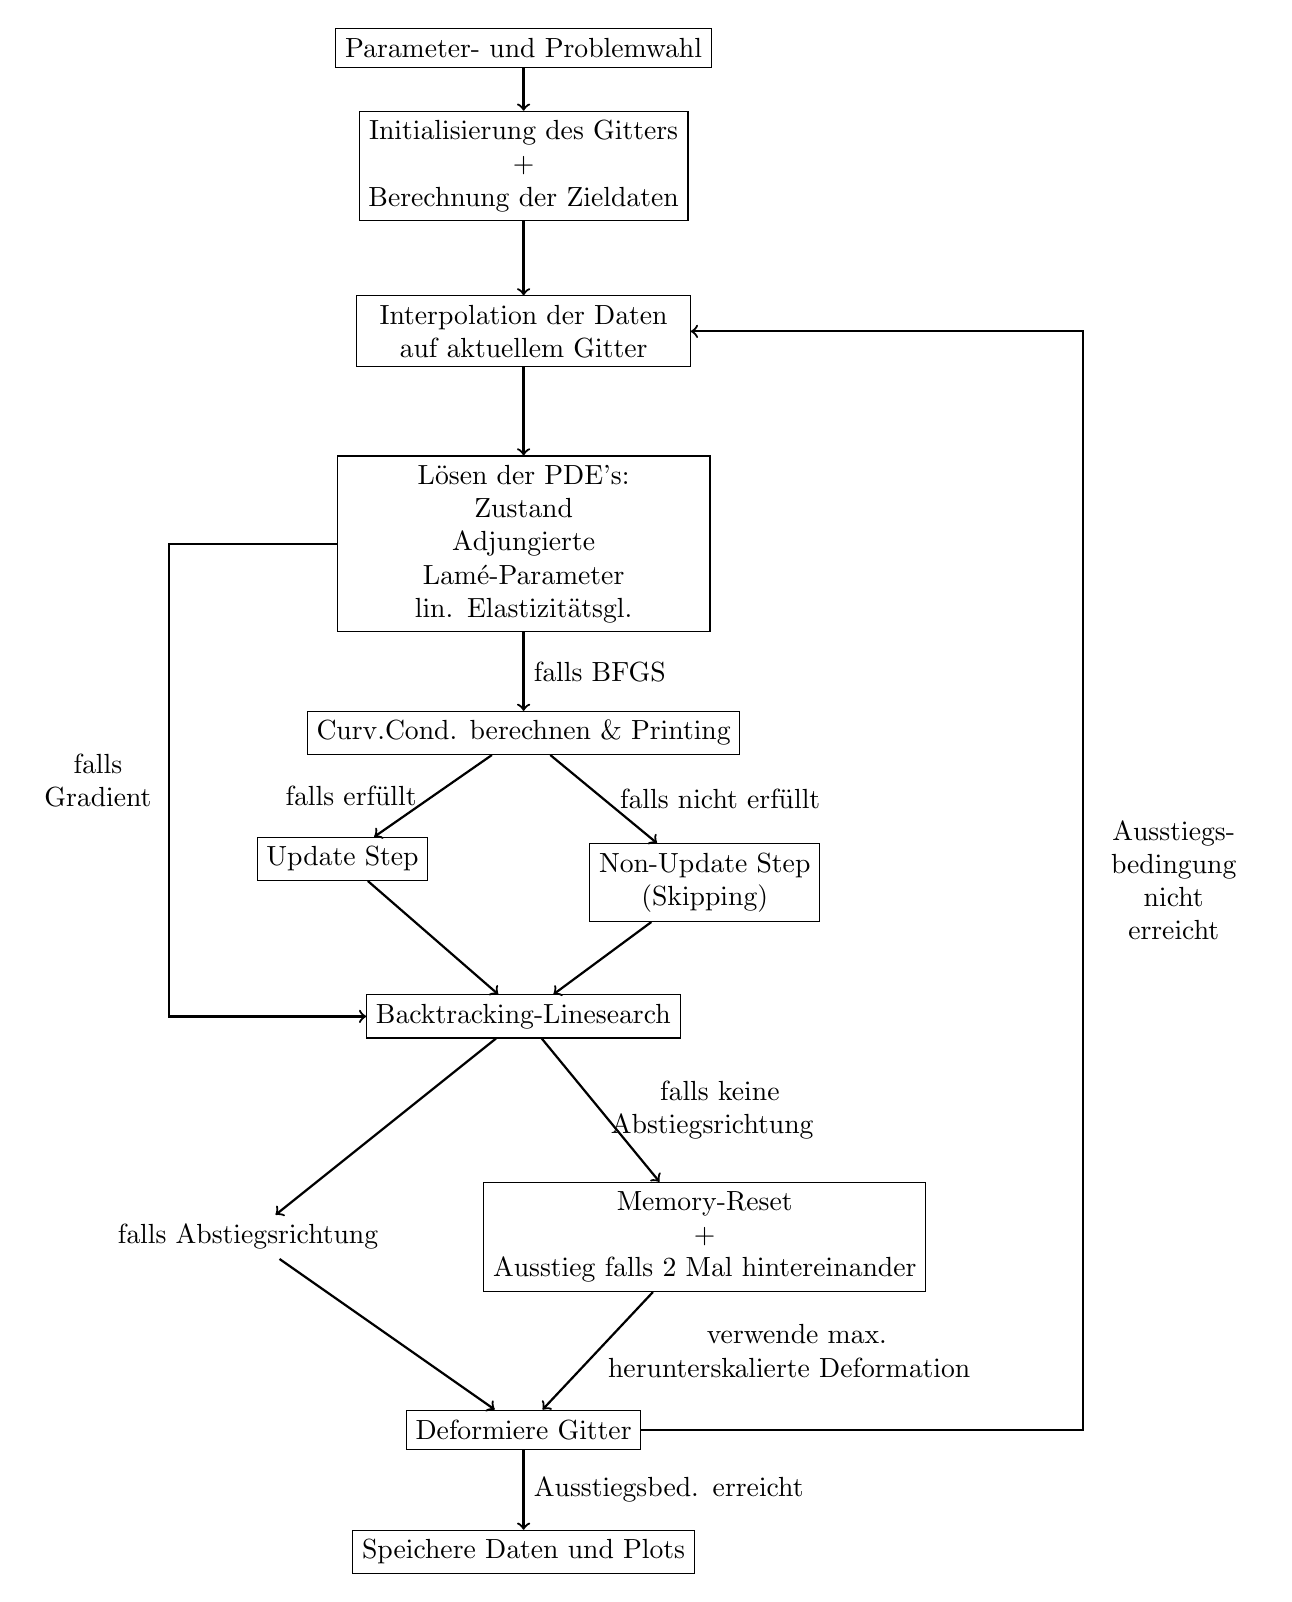
\begin{tikzpicture}
			\tikzstyle{sum} = [draw, circle, minimum size=0.8cm, node distance=1.75cm]
			\tikzstyle{block} = [draw, rectangle, minimum width = 2cm, minimum height = 0.5cm]
			\node [block, minimum width=1cm] (A) at (-3.5, 3.3) {Parameter- und Problemwahl}; 
			\node[block, fill=white, text width=4cm, align=center] (E) at (-3.5, -0.3) {Interpolation der Daten \\ auf aktuellem Gitter};
			\node[block, fill=white, align=center] (I) at (-3.5, 1.8) {Initialisierung des Gitters \\ + \\ Berechnung der Zieldaten};
			\draw[->,thick] (A) -- (I);
			\draw[->,thick] (I) -- (E);
			\node[block, fill=white, text width=4.5cm, align=center] (D) at (-3.5, -3) {L\"{o}sen der PDE's: \\
 Zustand \\
 Adjungierte \\
 Lamé-Parameter \\
 lin. Elastizit\"{a}tsgl.};
			\draw[->,thick] (E) -- (D);
			\node[block, fill=white] (F) at (-3.5, -5.4) {Curv.Cond. berechnen \& Printing};
			\draw[->,thick] (D) -- (F)  node[right, midway] {falls BFGS};
			\node[block, fill=white, text width=3.75cm] (G) at (-3.5, -9) {Backtracking-Linesearch};
			\node[block, fill=white] (J) at (-5.8, -7) {Update Step};
			\node[block, fill=white, align=center] (K) at (-1.2, -7.3) {Non-Update Step \\(Skipping)};
			\draw[->,thick] (F) -- (J) node [left, midway] {falls erf\"{u}llt\:};
			\draw[->,thick] (F) -- (K) node [right, midway] {\:falls nicht erf\"{u}llt};
			\draw[->,thick] (J) -- (G);
			\draw[->,thick] (K) -- (G);
			\node[block, fill=white] (H) at (-3.5, -14.25) {Deformiere Gitter};
			\node[block, fill=white, align=center] (N) at (-1.2, -11.8) {Memory-Reset \\ + \\ Ausstieg falls 2 Mal hintereinander};
			\node (O) at (-7, -11.8) {falls Abstiegsrichtung};
			\draw[->,thick] (G) -- (O);
			\draw[->,thick] (O) -- (H);
			\draw[->,thick] (N) -- (H) node [right,midway, align=center] {\: verwende max. \\ herunterskalierte Deformation};			
			\draw[->,thick] (G) -- (N) node [right,midway, align=center] {\: falls keine \\ Abstiegsrichtung}; 
			\draw[->,thick] (H.east) -- (3.6,-14.25) -- (3.6,-0.3) node[right, midway, text width=2.05cm, align=center] {Ausstiegs- \\ bedingung nicht \\ erreicht} -- (E.east);
			\draw[->,thick] (D.west) -- (-8,-3) -- (-8,-9) node[left, midway, text width=1.55cm, align=center] {falls \\ Gradient} -- (G.west);
			\node[block, fill=white] (L) at (-3.5, -15.8) {Speichere Daten und Plots};
			\draw[->,thick] (H) -- (L) node [right, midway, text width=4.5cm] {Ausstiegsbed. erreicht};
\end{tikzpicture}
\caption{Schematische Darstellung des Hauptprogramms \newline aus \textsf{shape\_main.py}}
\end{figure}
\newpage

Das Programm beginnt nach der Aktivierung über die Konsole mit der in \ref{meshdataclass} erklärten Initialisierung der Meshes. Je nach Einstellung findet die oben erklärte Pertubation des Startgitters statt. Weiterhin werden die lokal variierenden Lamé-Parameter, sowie die Zustandsfunktion im Zielgitter berechnet. Dies findet im Programm unter der Überschrift \textit{Targetdata Calculation} statt. Es folgt der Einstieg in den Formoptimierungsalgorithmus, wobei unter \textit{Interplation} die Daten auf das derzeitige Gitter zu einer FEniCS-Funktion interpoliert werden, für welche wir eine polynomielle Interpolation vom Grad 1 ausgewählt haben. Es werden anschließend die Zustands- und adjungierte Gleichung gelöst, sowie der Formgradient des derzeitigen Schrittes berechnet, was im Programm unter dem Schritt \textit{State, Adjoint \& Gradient Calculation} zu finden ist. Falls das Gradientenverfahren ausgewählt ist, wird zusätzlich als Deformation der negative Gradient initialisiert. 

Nun findet im Programm die Unterscheidung zwischen dem L-BFGS- und dem Gradientenverfahren statt; der folgende Abschnitt ist lediglich für das L-BFGS-Verfahren relevant, im Gradientenverfahren springt der Algorithmus direkt zu der Linesearch \ref{backtracking}.

Ein programmiertechnisch etwas aufwendiger Punkt ist die Berechnung der Curvature Condition. In unserem Setting ist diese errechnet durch 
\begin{equation}
\label{shapecurvcond}
\begin{aligned}
	a(S_k, \mathcal{T}_{S_k}^{-1}(\nabla U_{k+1}) - \nabla U_k) = D\mathcal{J}(\Omega_{k+1})[\mathcal{T}_{S_k}(S_k)] - D\mathcal{J}(\Omega_k)[S_k] > 0.
\end{aligned}
\end{equation}
Hierbei bedeutet $\mathcal{T}_{S_k}$ den Transport der Tangentialvektoren über die  Deformation $S_k$, ihr Inverses den Rücktransport, wie in Algorithmus \ref{2loopbfgs}. Dies vermeidet die Lösung einer weiteren linearen Elastizitätsgleichung, wobei wir wie angesprochen die vereinfachten Transporte aus \cite{diffusion}, Abschnitt 3, verwenden. Nichtsdestotrotz müssen wir zur Berechnung von $D\mathcal{J}(\Omega_{k+1})[\mathcal{T}_{S_k}(S_k)]$ eine Gitterverschiebung durchführen. Wir berechnen deshalb die Curvature Condition des $k$'ten Schrittes in Schritt Nummer $k+1$, da wir zuvor sowieso die passende Gitterverschiebung durchführen mussten. Die Deformation $S_k$ aus dem Schritt $k$ wird im Programm unter \textsf{last\_defo} mitgeschleppt, der Wert der Ableitung $D\mathcal{J}(\Omega_k)[S_k]$ als Eintrag \textsf{curv\_cond[1]} gespeichert. Wir wählen diese kompliziert wirkende Iteration, um zu häufiges verschieben der Meshes zu vermeiden, denn FEniCS verschiebt auch das Ausgangsgitter, wenn ein anderes Gitter unter selber Initialisierung verschoben wird. Dies könnte man vermeiden, indem man eine Deep Copy anlegt, was bei großen Gittern speicherintensiv sein kann. Hinzu kommen Rundungsfehler, deren Ausmaß wir jedoch nicht einschätzen können.
Als Folge der um einen Schritt verschobenen Berechnung printen wir im L-BFGS-Verfahren die Werte der Schleife $k$ in Schleife $k+1$, außerdem wird die Memory aus selbigen Gründen erst dann geupdatet. Bei Einhaltung der Curvature Condition findet der Update unter dem Abschnitt \textit{Update Step} statt, das Printen und die Berechnung der Curvature Condition unter dem Abschnitt \textit{Curvature Condition \& Printing}. 

Im Falle, dass die Curvature Condition \ref{shapecurvcond} nicht erfüllt ist, verwenden wir das Verfahren, die Memory nicht einem Update zu unterziehen, d.h. es wird lediglich ein Schritt mit schon vorhandenen Daten berechnet und angewandt. Dieses Skipping findet im Programm unter dem Abschnitt \textit{Non Update Step} statt. Da der Update sowieso einen Schritt verzögert stattfindet, wird dieser einfach ausgelassen, und das Programm läuft weiter. Diese Strategie lässt sich mit der Einstellung des Parameter \textsf{curv\_break = True} ausschalten, woraufhin der Algorithmus bei Verletzung der Curvature Condition aussteigt.

\subsubsection{Die Backtracking-Linesearch}
\label{backtracking}
Nachdem die Gradienten und Deformationen berechnet wurden, erfolgt je nach Einstellung eine Linesearch mittels Backtracking. Diese wird gesteuert durch die Parameter \textsf{Linesearch}, \textsf{shrinkage}, \textsf{c} und \textsf{start\_scale}. Ersterer schaltet die Linesearch bei \textsf{Linesearch = True} ein, \textsf{shrinkage} ist der Reskalierungsfaktor bei einem Backtracking-Schritt, \textsf{c} gibt den Faktor der Verbesserung im Zielfunktional im Vergleich zum derzeitigen Wert an, und \textsf{start\_scale} gibt den Faktor zur Hochskalierung zum Beginn des Backtracking an.

Die Linesearch startet mit dem Berechnen der hochskalierten Deformation.
\begin{lstlisting}
if(Linesearch):
	scale_parameter = start_scale

    zero_function = Function(VectorFunctionSpace(MeshData.mesh,
                                                 "P", 1, dim=2))
    current_value = bib.targetfunction(MeshData, zero_function,
        								               y_z, f_values, nu)
    S.vector()[:] = start_scale * S.vector()
    current_deriv = bib.shape_deriv(MeshData, p, y, z, 
    								                f_values, nu, S)

    counterer = 0
\end{lstlisting}
Der Counter \textsf{counterer} zählt dabei die Anzahl der Reskalierungen der Deformation. Das eigentliche Backtracking findet in der gleich folgenden Schleife statt. Weiterhin ist in dieser Schleife die Strategie implementiert, bei maximalem Herunterskalieren des Deformationsfeldes die L-BFGS-Memory zu löschen und das Verfahren im jetzigen Punkt neu zu starten, wobei dies mit einer Meldung zur Kenntnis gegeben wird. Falls das Verfahren im sofort darauf folgenden Schritt erneut maximal herunterskaliert, wird das Optimierungsverfahren mit einer Fehlermeldung abgebrochen. Hierzu wird der Counter \textsf{Resetcounter} verwendet.

\begin{lstlisting}
while(bib.targetfunction(MeshData, S, y_z, f_values, nu)
       >= current_value):
	
	scale_parameter = shrinkage * scale_parameter
    S.vector()[:]   = shrinkage * S.vector()

    counterer = counterer + 1

	if(counterer >= 20):
    	print("Had to break, restarting L-BFGS!")

        bfgs_memory.gradient    = np.zeros([memory_length, 2 * 																     MeshData.mesh.num_vertices()])
        bfgs_memory.deformation = np.zeros([memory_length, 2 * 																   MeshData.mesh.num_vertices()])
        bfgs_memory.step_nr     = 0
        Resetcounter            = Resetcounter + 1
        S.vector()[:]           = np.zeros(2*MeshData.mesh.
        											           num_vertices())
        break

        if(counterer < 20):
            Resetcounter = 0

        last_defo = S.vector().get_local()

if(Resetcounter >= 2):
    print("Reboot didn't help, quitting L-BFGS optimization!")
    break
\end{lstlisting}

Es ist außerdem möglich, statt der einfachen Backtrackingbedingung, die sogenannte \textit{Armijo-Bedingung} mit Hilfe eines Backtracking-Verfahrens zu implementieren, siehe \cite{Nocedal}, Gleichung (3.4).
Dies würde mit einer Schleife der Form
\begin{lstlisting}
while(bib.targetfunction(MeshData, S, y_z, f_values, nu)
       > current_value + c*scale_parameter*current_deriv):
		#Schleifenaktionen von oben
\end{lstlisting}
funktionieren, wobei der Befehl \textsf{targetfunction} den Wert des Zielfunktionals im Gitter berechnet, welches durch Verschieben mit der Deformation \textsf{S} entsteht, und dieses wieder zurück deformiert. Diese Schleife haben wir in auskommentierter Form im Code eingefügt, so dass der Benutzer diese durch entfernen der Auskommentierung verwenden kann.

An dieser Stelle sei erwähnt, dass wir die nach \cite{Powell}, Abschnitt 5, beschriebene Methode zur Einhaltung der Curvature Condition versucht haben zu implementieren. Dieses Verfahren wird \textit{Powell-Relaxation} genannt, und ersetzt mit Hilfe eines Kriteriums, welches die BFGS-Approximierende $B_k$ aus Definition \ref{BFGS-updates} zur Berechnung verwendet, die Differenz der Gradienten $y_k$ aus Definition \ref{BFGS-updates}. Das die Differenz der Gradienten ersetzende Vektorfeld würde dann die Curvature Condition erfüllen, und somit ein positiv definiten Update $B_{k+1}$ garantieren. Zum einen haben wir dies nicht implementiert, da zur Berechnung $B_k$ selbst benötigt würde, wir aber den 2-Schleifen-Algorithmus \ref{2loopbfgs} verwenden, um lediglich die Anwendung der Inversen $B_k^{-1}$ zu berechnen. Weiterhin führt dieses Verfahren zu einem sogenannten \textit{Blow-Up} der Hesse-Approximation, weshalb das Verfahren dann neu gestartet werden müsste, und somit sich die Frage nach dem Nutzen im Vergleich zum Aufwand stellt. Aus diesen Gründen haben wir die Powell-Relaxation nicht implementiert.

\subsubsection{Der Output}
Abschließend kommen wir im Kapitel der Implementierung zum Output des Programms.
Zu Beginn wird bei Aufruf des Programms ein Outputordner im Verzeichnis des Programms mit Namen \textsf{Output} erzeugt, falls dieser noch nicht vorhanden ist. Dies geschieht mit der implementierten Funktion \textsf{create\_outputfolder()}. In diesen Ordner wird für jedes Aufrufen des Programms, sprich für jedes Optimierungsproblem, ein eigener Unterordner mit dem Namen erstellt, welcher nach dem exakten jetzigen Datum bis auf die Sekunde benannt wird. Beispielsweise würde ein Outputordner, welcher am 11.09.2001 um 8:46 und 0 Sekunden erzeugt wurde, den Namen 
\begin{center}
\textsf{20010911\_084600}.
\end{center}
erhalten. Dadurch wird immer ein eindeutig bestimmter, neuer Outputordner erzeugt. In diesem werden die Gitter der einzelnen Iterationen mit den zugehörigen Formen, sowie die Daten des Zielgitters in \textsf{.pvd}-Dateien gespeichert, welche beispielsweise mit dem Programm \textit{Paraview}\footnote{Wir verwenden für die Erzeugung der Bilder im nächsten Kapitel Paraview 5.0.1.} visualisiert werden können. Zusätzlich wird bei erfolgreichem Durchlaufen der Optimierung ein Konvergenzplot gespeichert, welcher die Abbildungen
\begin{align*}
k &\mapsto \log(d_{shopt}(\Omega_k, \Omega_{target}) \\
k &\mapsto \log(\vert\vert D\mathcal{J}(\Omega_k) \vert\vert)
\end{align*}
zeigt, wobei die Norm wie unter \ref{felas} erklärt berechnet wird. Um eine Analyse der Verfahren besser durchführen zu können, werden weiterhin relevante Größen in einer \textsf{.cvd}-Datei gespeichert. Diese Daten werden in der selben Anordnung gespeichert, wie sie im Laufe des Programms auch für den Benutzer in der Konsole geprintet werden. Schematisch sieht dies wie folgt aus:
\begin{center}
\textsf{Iteration \hspace{0.1cm}  ||f\_elas||\_L2 \hspace{0.1cm}  J = j + j\_reg   \hspace{0.1cm} ||U||\_L2 \hspace{0.1cm}  Curv. Cond. \hspace{0.1cm} Meshdistance}
\end{center}

Falls das Gradientenverfahren ausgewählt wurde, so wird die Spalte mit der Curvature Condition weggelassen. Diese Datei lässt sich im Rahmen des Postprocessings bequem mit Programmen wie \textit{Excel} oder \textit{RStudio} bearbeiten. Sollte das Verfahren divergieren, etwa falls die Curvature Condition einige Schritte nicht erfüllt ist, so findet keine Speicherung der Konvergenzgraphen statt. Die \textsf{.pvd}-Dateien werden trotzdem gespeichert, die \textsf{.csv}-Datei ist leer, wobei man dies durch Erstellen und Speicherung einer neuen \textsf{.csv}-Datei in jedem Schritt umgehen könnte. 
Im nun folgenden und letzten Kapitel werden wir solche Analysen für einige von uns ausgewählte Routinen vorstellen.

